
\documentclass[journal, onecolumn, 10pt]{IEEEtran}

% correct bad hyphenation here
\hyphenation{op-tical net-works semi-conduc-tor}

\usepackage{graphicx}
\usepackage{subfig}
\usepackage{amssymb}
\usepackage{amsmath} 
\usepackage[colorlinks,linkcolor=red]{hyperref}
\begin{document}

% Do not put math or special symbols in the title.
\title{Final Project of ELEC5470 FALL 2017 \\ Optimization in Image Deblurring \\ Initial Proposal}

\author{Xiaoyun~Yuan,~20322404}


% The paper headers
\markboth{ELEC5470 Final Project Xiaoyun Yuan}%
% The only time the second header will appear is for the odd numbered pages
{}
% make the title area
\maketitle

% As a general rule, do not put math, special symbols or citations
% in the abstract or keywords.
\begin{abstract}
In this report , I present some representative image deblurring algorithms and the convex/non-convex optimization techniques used in these papers. 
\end{abstract}

% Note that keywords are not normally used for peerreview papers.
\begin{IEEEkeywords}
Optimization, Image Deblurring, Prior 
\end{IEEEkeywords}

% For peerreview papers, this IEEEtran command inserts a page break and
% creates the second title. It will be ignored for other modes.
\IEEEpeerreviewmaketitle

\section{Introduction}
Nowadays, smart phone has become the digital hub of everyone's daily life, and camera is one of the most important modules on smart phones. However, limited by the space of smart phones, the smart phone camera optic system is often very simple and CMOS size is usually very small. That means the image quality is easily affected environment, for example, low light condition leads to severe noise, camera shaking and long exposure time causes uncomfortable blur effect. In this report, I focus on how to remove the image blur effects caused by camera shaking.

Image deblurring is a fundamental computer vision research problem. Now, there are two different ways to solve the image deblurring problem: 1) traditional convolutional model approach; 2) neural network approach. In this report, I mainly focus on the first approach and give some brief introductions of the second approach.

\subsection{Traditional Convolutional Model Approach}
In traditional convolutional model, the image blur effect is expressed by $2D$ convolution:
\begin{equation}
\mathbf{b} = \mathbf{l} \otimes \mathbf{k} + \mathbf{n},
\label{eqn:convolutional_blur_model}
\end{equation}
where $\mathbf{b}$, $\mathbf{l}$ and $\mathbf{k}$ are the blurry image, latent sharp/unblurred image and blur kernel respectively. $\mathbf{n}$ denotes the noise. The blur kernel $\mathbf{k}$ is usually expressed by a small matrix which is related to the camera shaking trajectory, as shown in the Fig.~\ref{fig:convolutional_blur_model}. Because the 2D convolution is difficult to handle, Eqn.~\ref{eqn:convolutional_blur_model} is often written in frequency domain:
\begin{equation}
\mathcal{F}(\mathbf{b}) = \mathcal{F}(\mathbf{l}) \cdot \mathcal{F}(\mathbf{k}) + \mathcal{F}(\mathbf{n}),
\label{eqn:convolutional_blur_model_frequency}
\end{equation}
where $\mathcal{F}(\cdot)$ denotes the Fourier transform.
\begin{figure}[h!]
\centering
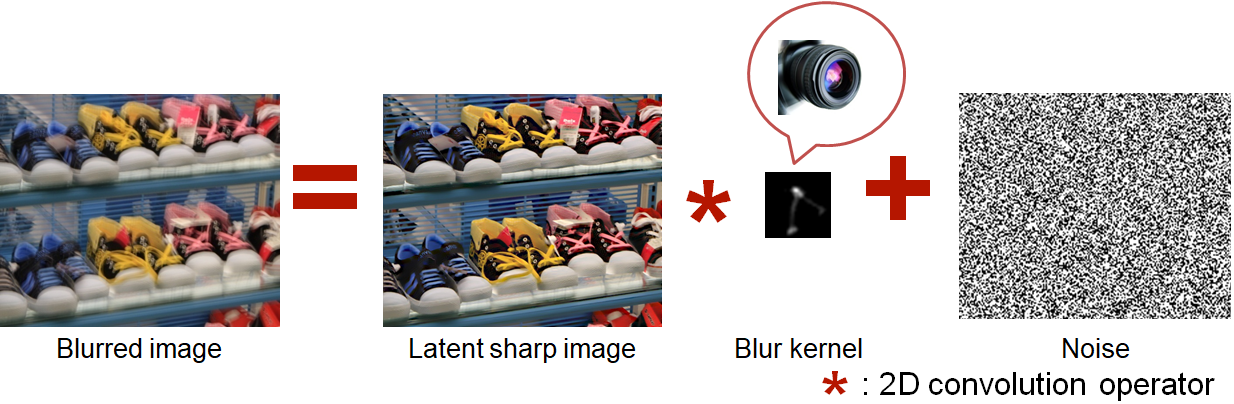
\includegraphics[width = 1\textwidth]{pic/convolutional_model.png}
\caption{Image Convolutional Blur Model}
\label{fig:convolutional_blur_model}
\end{figure}

The deblurring problem can be divide into two kinds: 1) non-blind deblurring: only $\mathbf{l}$ is unknown, use existing $\mathbf{k}$ to solve latent sharp image $\mathbf{l}$:
\begin{equation}
\min_{\mathbf{l}} \| \mathbf{b} - \mathbf{l} \otimes \mathbf{k} \|.
\label{eqn:non_blind_origin}
\end{equation}
2) Blind deblurring: both $\mathbf{l}$ and $\mathbf{k}$ are unknown:
\begin{equation}
\min_{\mathbf{l}, \mathbf{k}} \| \mathbf{b} - \mathbf{l} \otimes \mathbf{k} \|,
\label{eqn:blind_origin}
\end{equation}

The non-blind deblurring looks easy, but in fact, it is very tough in image deblurring problems. I recommend the readers to read the simple introduction \cite{deblurintro}\url{https://blogs.mathworks.com/steve/2007/08/13/image-deblurring-introduction/} first. The results are shown in Fig.~\ref*{fig:simple_inverse_filter}: (a) and (d) show the blurry image and groundtruth image respectively. (b) is the deblurring result using pseudo inverse filter. We can see that although the main structure of the image is recovered, a lot of artifacts (ringing and noise) are introduced. (c) is the result of the state-of-the-art non blind deblurring algorithm \cite{krishnan2009fast}, which I will introduce in next section.

\begin{figure}[h!]
\centering
\subfloat[blurry image and kernel]{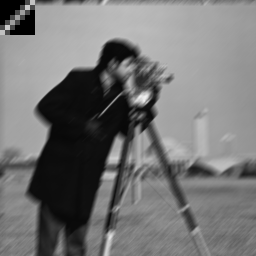
\includegraphics[width = 0.23\textwidth]{pic/cameraman_blur.png}}
\hspace{\fill}
\subfloat[pseudo inverse filter]{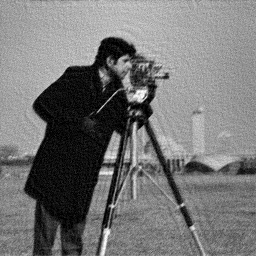
\includegraphics[width = 0.23\textwidth]{pic/cameraman_blur_pseudo_inverse.png}}
\hspace{\fill}
\subfloat[hyper laplacian $\|\nabla \mathbf{l} \|_{0.5}$\cite{krishnan2009fast}]{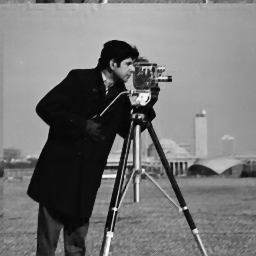
\includegraphics[width = 0.23\textwidth]{pic/cameraman_hyper_laplacian.png}}
\hspace{\fill}
\subfloat[groundtruth image]{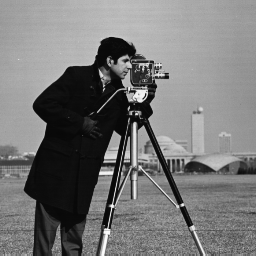
\includegraphics[width = 0.23\textwidth]{pic/cameraman.png}}
\hspace{\fill}
\caption{Image Deblurring Example}
\label{fig:simple_inverse_filter}
\end{figure}

To solve the problem is Fig.~\ref*{fig:simple_inverse_filter}(b), existing state-of-the-art algorithms usually solve the following optimization problem with image prior $\phi$ and kernel prior $\rho$ instead of original one: 1) Non-blind deblurring
\begin{equation}
\min_{\mathbf{l}} \| \mathbf{b} - \mathbf{l} \otimes \mathbf{k} \| + \lambda\phi(\mathbf{l}).
\label{eqn:non_blind_with_prior}
\end{equation}
2) Blind deblurring
\begin{equation}
\min_{\mathbf{l}, \mathbf{k}} \| \mathbf{b} - \mathbf{l} \otimes \mathbf{k} \| + \lambda\phi(\mathbf{l}) + \mu \rho(\mathbf{k}).
\label{eqn:blind_with_prior}
\end{equation}

Usually, Eqn.~\ref{eqn:blind_with_prior} will be split into two minimization problems and solve  $\mathbf{l}$ and $\mathbf{k}$ alternatively:
\begin{equation}
\begin{cases}
\min_{\mathbf{l}}&\| \mathbf{b} - \mathbf{l} \otimes \mathbf{k} \| + \lambda\phi(\mathbf{l}) \\
\min_{\mathbf{k}}&\| \mathbf{b} - \mathbf{l} \otimes \mathbf{k} \| + \mu \rho(\mathbf{k})
\end{cases}
\label{eqn:blind_with_prior_alternative}
\end{equation}
Nowadays, the image are very large. For example, a smart phone with $12$MP could capture $3968 \times 2976$ images, which means usually very large kernels are needed to estimate (larger than $120 \times 120$). To directly estimate a variable with so high dimension is very difficult, so most blind deblurring algorithms choose a multi-scale coarse-to-fine approach: estimating a smalling kernel using low resolution image first and resizing to high resolution as the initial value.


\subsection{Neural Network Approach}
The convolutional model looks very beautiful, but solving it is really not easy. Therefore, some researchers proposed to use neural network to predict the latent sharp image directly. For example, the neural network in Fig.~\ref{fig:deep_video_deblurring_cnn} takes the stacked nearby videos frames as input, and directly output the deblurred central video. 

\begin{figure}[h!]
\centering
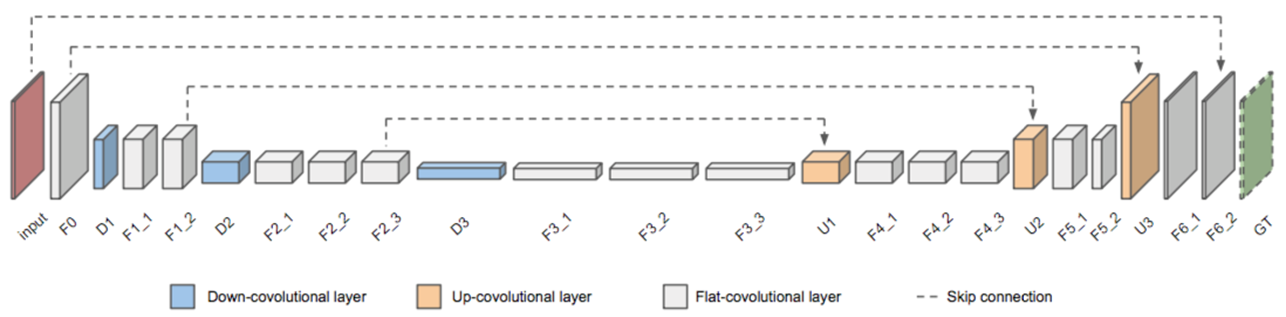
\includegraphics[width = 1\textwidth]{pic/deep_video_deblurring_cnn.png}
\caption{Structure of CNN used in Deep Video Deblurring\cite{su2016deep}}
\label{fig:deep_video_deblurring_cnn}
\end{figure}

Until now, the neural network is still a black box to researchers. No one could give a theoretical explanation, so I am not going to talk the details here.

\section{Overview of Existing Work}
In this section, I categorize the deblurring algorithms into $3$ kinds: 1) image priors; 2) kernel priors; 3) neural networks priors, and briefly introduce some representative works in this section.

\subsection{Image Priors}
\label{subsec:image_prior}
As mentioned above, I formulate the image deblurring objective function as following minimization problem:
\begin{equation}
\min_{\mathbf{l}, \mathbf{k}} \| \mathbf{b} - \mathbf{l} \otimes \mathbf{k} \| + \lambda\phi(\mathbf{l}) + \mu \rho(\mathbf{k}).
\label{eqn:objective_funtion}
\end{equation}
~\\
\textbf{\emph{Hyper-laplacian Prior}}\cite{krishnan2009fast}: this paper proposed a excellent non-blind image deblurring algorithm. Kernel is already given in non-blind deblurring so only need to solve the first problem in Eqn.~\ref{eqn:blind_with_prior_alternative}. A hyper-laplacian image prior $\phi(\mathbf{l}) = \|\nabla \mathbf{l}\|_{\alpha}$ is proposed in this paper. As shown in Fig.~\ref{fig:hyper_laplacian}, the dark blue curve denotes the empirical image gradient distribution of natural images. The reason why hyper-laplacian is proposed is that the curve shape of  hyper-laplacian (green) is closet to the empirical one (dark blue). 
\begin{figure}[h!]
\centering
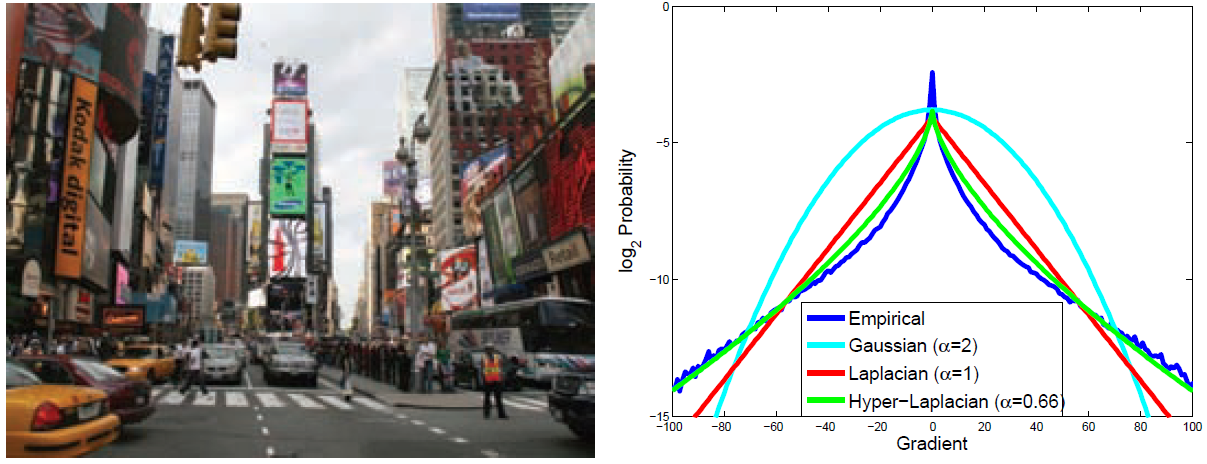
\includegraphics[width = 1\textwidth]{pic/hyper_laplacian.png}
\caption{Hyper-Laplacian Image Prior\cite{su2016deep}}
\label{fig:hyper_laplacian}
\end{figure}

However, solving the problem is still not trivial because the image prior $\phi(\mathbf{l}) = \|\nabla \mathbf{l}\|_{\alpha}$ is non-convex. The most commonly used method in image deblurring is to re-formulate the objective function again:
\begin{equation}
\min_{\mathbf{l}} \| \mathbf{b} - \mathbf{l} \otimes \mathbf{k} \|_2^2 + \lambda_1 \|\nabla \mathbf{l} - \mathbf{g}\|_2^2 + \lambda_2\|\mathbf{g}\|_{\alpha}.
\label{eqn:hyper_laplacian}
\end{equation}
Eqn.~\ref{eqn:hyper_laplacian} can be divided into two sub-optimization problems and solve alternatively:
\begin{equation}
\begin{cases}
\min_{\mathbf{l}} &\| \mathbf{b} - \mathbf{l} \otimes \mathbf{k} \|_2^2 + \lambda_1 \|\nabla \mathbf{l} - \mathbf{g}\|_2^2 \\
\min_{\mathbf{g}} &\lambda_1\|\nabla \mathbf{l} - \mathbf{g}\|_2^2 + \lambda_2\|\mathbf{g}\|_{\alpha}.
\end{cases}
\label{eqn:hyper_laplacian_alter}
\end{equation}
The first minimization problem if Eqn.~\ref{eqn:hyper_laplacian} is a least-square problem which has closed-form solution:
\begin{equation}
\mathbf{l} = \mathcal{F}^{-1} \left( \frac{\overline{\mathcal{F}(\mathbf{k})}\mathcal{F}(\mathbf{b}) + \lambda_1F_G}
{\overline{\mathcal{F}(\mathbf{k})}\mathcal{F}(\mathbf{k}) + \lambda_1\overline{\mathcal{F}(\nabla)}\mathcal{F}(\nabla)} \right),
\label{eqn:l2_latent_close_form}
\end{equation}
where $F_G = \overline{\mathcal{F}(\nabla_h)}\mathcal{F}(\mathbf{g}_h) + \overline{\mathcal{F}(\nabla_v)}\mathcal{F}(\mathbf{g}_v)$. $\nabla_h$ and $\nabla_v$ represent the horizontal and vertical differential operators.
The second problem is difficult, exact analytical solutions can only be found for some specific value, e.g. $\alpha = 0.5, 0.66$. For general $\alpha$ values, this paper proposed a lookup table solution.

~\\
\textbf{\emph{Unnatural $L_0$ Sparsity Prior}}\cite{xu2013unnatural}: this paper proposed a blind image blurring algorithm with objective function as follows:
\begin{equation}
\min_{\mathbf{l}, \mathbf{k}} \| \mathbf{b} - \mathbf{l} \otimes \mathbf{k} \|_2^2 + \lambda \|\nabla \mathbf{l} \|_0 + \mu \| \mathbf{k} \|_2^2.
\label{eqn:l0_sparse}
\end{equation}
Similar as the hyper-laplacian prior paper, this large optimization problem can be re-formulated into 3 small sub-problems and solved alternatively. The kernel is estimated in gradient space $\nabla\mathbf{l}$, $\nabla\mathbf{b}$ to replace $\mathbf{l}$, $\mathbf{b}$, because estimating kernel in gradient space is more accurate\cite{cho2009fast}.
\begin{equation}
\begin{cases}
\min_{\mathbf{l}} &\| \mathbf{b} - \mathbf{l} \otimes \mathbf{k} \|_2^2 + \lambda_1 \|\nabla \mathbf{l} - \mathbf{g}\|_2^2 \\
\min_{\mathbf{g}} &\lambda_1\|\nabla \mathbf{l} - \mathbf{g}\|_2^2 + \lambda_2\|\mathbf{g}\|_{0} \\
\min_{\mathbf{k}} &\| \nabla\mathbf{b} - \nabla\mathbf{l} \otimes \mathbf{k} \|_2^2 + \mu \|k\|_2^2.
\end{cases}
\label{eqn:l0_sparse_alter}
\end{equation}
The first sub-problem is same as the Eqn.~\ref{eqn:hyper_laplacian_alter}. The third sub-problem also has closed form solution:
\begin{equation}
\mathbf{k} = \mathcal{F}^{-1} \left( \frac{\overline{\mathcal{F}(\nabla_h\mathbf{l})}\mathcal{F}(\nabla_h\mathbf{b}) + 
\overline{\mathcal{F}(\nabla_v\mathbf{l})}\mathcal{F}(\nabla_v\mathbf{b})}
{\overline{\mathcal{F}(\nabla_h\mathbf{l})}\mathcal{F}(\nabla_h\mathbf{l}) + 
\overline{\mathcal{F}(\nabla_v\mathbf{l})}\mathcal{F}(\nabla_v\mathbf{l}) + \mu} \right).
\label{eqn:l2_kernel_close_form}
\end{equation}
Sometimes, the close form solution is not stable, conjugate gradient method can be used to estimate a more stable result.

The key contribution of this paper is to solve the second sub-problem of Eqn.~\ref{eqn:l0_sparse_alter}. This paper proposed an easy and quick close form solution (the proof is in the supplementary material of \cite{xu2013unnatural}):
\begin{equation}
\mathbf{g}_i = 
\begin{cases}
\nabla\mathbf{l}_i, &~~ |\nabla\mathbf{l}_i|^2 \geqslant \frac{\lambda_2}{\lambda_1}, \\
0, &~~ \text{otherwise}.
\end{cases}
\end{equation}

~\\
\textbf{\emph{$L_0$ Regularized Intensity and Gradient Prior}}\cite{pan2014deblurring}: an extension of unnatural $L_0$ sparsity prior\cite{xu2013unnatural} used for text image deblurring: $\phi(\mathbf{l}) = \alpha\| \mathbf{l} \|_0 + \|\nabla \mathbf{l} \|$. The solving method is nearly the same as that in \cite{xu2013unnatural}, only needs more iterations to refine $\mathbf{l}$ and $\mathbf{\nabla \mathbf{l}}$ alternatively.

~\\
\textbf{\emph{Normalized Sparsity Prior $L_1/L_2$}} \cite{krishnan2011blind}: this paper proposed a image prior called normalized sparsity prior $\phi(\mathbf{l}) = \frac{\|\nabla\mathbf{l}\|_1}{\|\nabla\mathbf{l}\|_2}$, and the objective function becomes:
\begin{equation}
\min_{\mathbf{l}, \mathbf{k}} \|\mathbf{b} - \mathbf{l} \otimes \mathbf{k} \|_2^2 + \lambda \frac{\|\nabla\mathbf{l}\|_1}{\|\nabla\mathbf{l}\|_2} + \mu \|\mathbf{k}\|_1.
\label{eqn:normalized_sparisty}
\end{equation}
The reason why use normalize sparsity as image prior is that $L_1/L_2$ is a quite good measure of image sharpness, as shown in Fig.~\ref{fig:normalized_sparisty}.
\begin{figure}[h!]
\centering
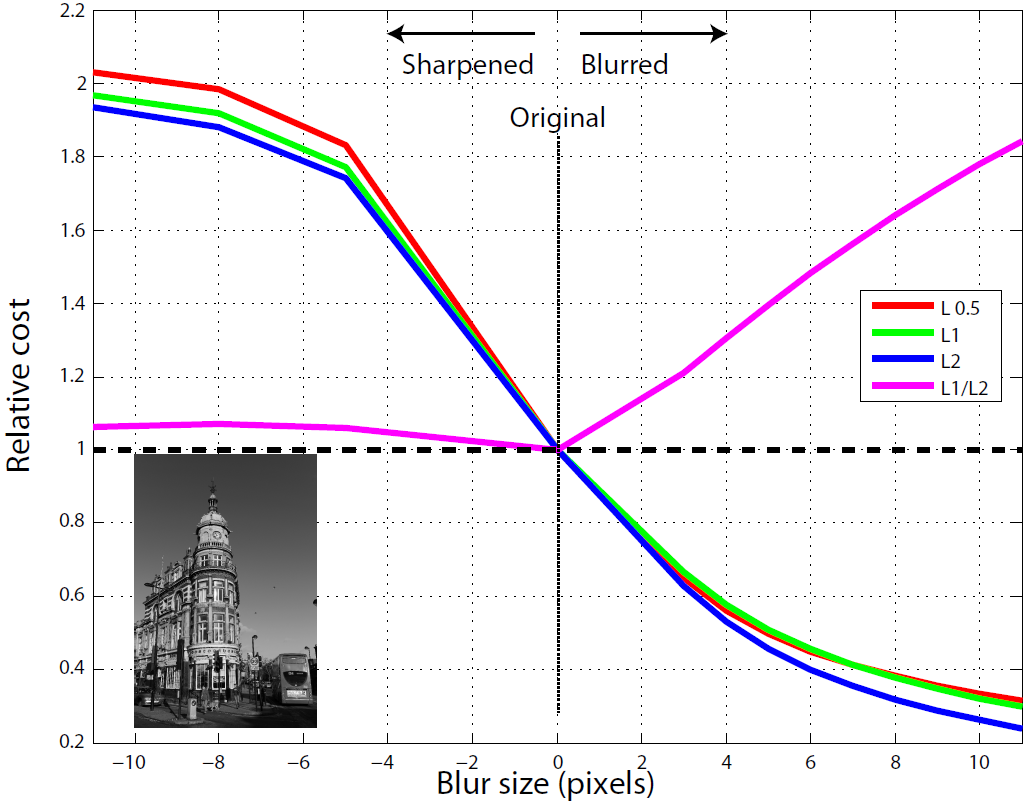
\includegraphics[width = 0.5\textwidth]{pic/normalized_sparsity.png}
\caption{Normalized Sparsity Measure $\frac{L_1}{L_2}$}
\label{fig:normalized_sparisty}
\end{figure}

Similarly, Eqn.~\ref{eqn:normalized_sparisty} can be divide into the following two sub-problems:
\begin{equation}
\begin{cases}
\min_{\mathbf{l}} &\| \mathbf{b} - \mathbf{l} \otimes \mathbf{k} \|_2^2 + \lambda_1 \frac{\|\nabla\mathbf{l}\|_1}{\|\nabla\mathbf{l}\|_2} \\
\min_{\mathbf{k}} &\| \nabla\mathbf{b} - \nabla\mathbf{l} \otimes \mathbf{k} \|_2^2 + \mu \|k\|_1.
\end{cases}
\label{eqn:normalized_sparsity_alter}
\end{equation}
Different from the above mentioned papers, $L_1$ norm is used here to estimate kernel. No close form solution but it can be solved by iterative re-weighted least squares (IRLS) easily. The first sub-problem is non-convex and very difficult to solve directly. To make it solvable, this paper design an iterative optimization algorithm with inner and outer loops: in inner loop, first fix the denominator $\|\nabla \mathbf{l}\|_2$ and this problem becomes a convex $L_1$ regularized problem which can be solved by iterative shrinkage-thresholding algorithm (ISTA)\cite{beck2009fast}. In outer loop, re-estimate the denominator $\|\nabla \mathbf{l}\|_2$.

\subsection{Kernel Priors}
\label{subsec:kernel_prior}
All the papers in Section.~\ref{subsec:image_prior} use very simple kernel prior ($\|k\|_2^2$ or $\|k\|_1$), which are convex and very easy to solve. However, it is not good enough sometimes, as illustrated in Fig.~\ref{fig:kernel_noise}. Small noise or fake branches in kernel can cause severe visual artifacts.
\begin{figure}[h!]
\centering
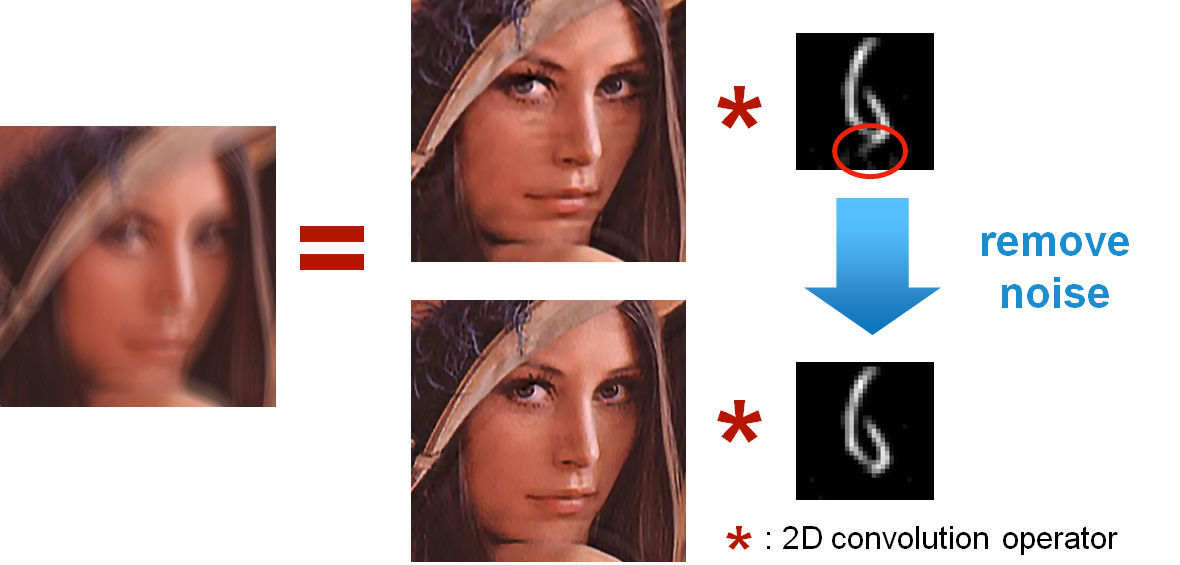
\includegraphics[width = 0.7\textwidth]{pic/kernel_noise.png}
\caption{Effect of Kernel Noise}
\label{fig:kernel_noise}
\end{figure}
Therefore, some paper propose specific kernel prior, for example, using IMU (inertial measurement sensor) to help estimate the kernel shape. In this report, we introduce a simple optimization based approach:

~\\
\textbf{\emph{Separable Kernel Prior}}\cite{fang2014separable}: this paper proposed to force the kernel in a curve region by extract the trajectory of the kernel, and the original kernel optimization sub-problem becomes
\begin{equation}
\begin{cases}
\min_{\mathbf{K}} &\|\nabla\mathbf{b} - \nabla\mathbf{l} \otimes \mathbf{k} \|_2^2 + \mu \|W \odot \mathbf{k} \|_1 \\
\text{s.t.}~~ &W = 1 - E(T).
\end{cases}
\label{eqn:normalized_sparsity_alter}
\end{equation}
\begin{figure}[h!]
\centering
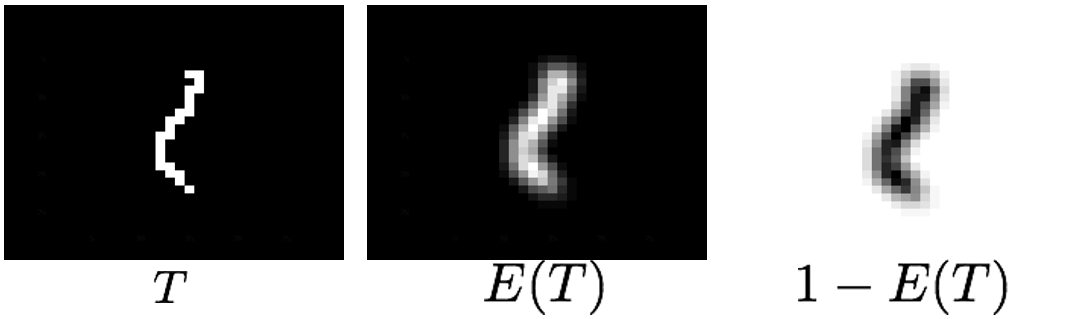
\includegraphics[width = 0.5\textwidth]{pic/separable_kernel.png}
\caption{Refine Kernel Estimation using Trajectory}
\label{fig:separable_kernel}
\end{figure}

As presented in Fig.~\ref{fig:separable_kernel}, where $odot$ is element-wise product, $T$ denotes the trajectory of the original kernel, $E(\cdot)$ represent the Gaussian mask and $W$ is the mask used to remove noise and fake branches in kernel.

\subsection{Neural Networks Priors}
\label{subsec:neural_network_prior}
The image priors proposed in Section.~\ref{subsec:image_prior} are very simple statistics, which can be solved by existing optimization techniques but have many failure cases unavoidably. Thus, some researchers proposed to use neural network as image prior. In this report, I introduce a non-iterative neural approach.

~\\
\textbf{\emph{Non-iterative Neural Approach}}\cite{chakrabarti2016neural}: the methods in Section.~\ref{subsec:image_prior} derive latent sharp image $\mathbf{l}$ update rule from objective functions and the image priors are used as an image sharpness measure. However, it is infeasible for neural network priors because of its high-complexity. Therefore, this paper proposed to train a neural network to update the latent sharp image  $\mathbf{l}$ directly, as shown in Fig.~\ref{fig:non_iterative_nn}.
\begin{figure}[h!]
\centering
\subfloat[pipeline]{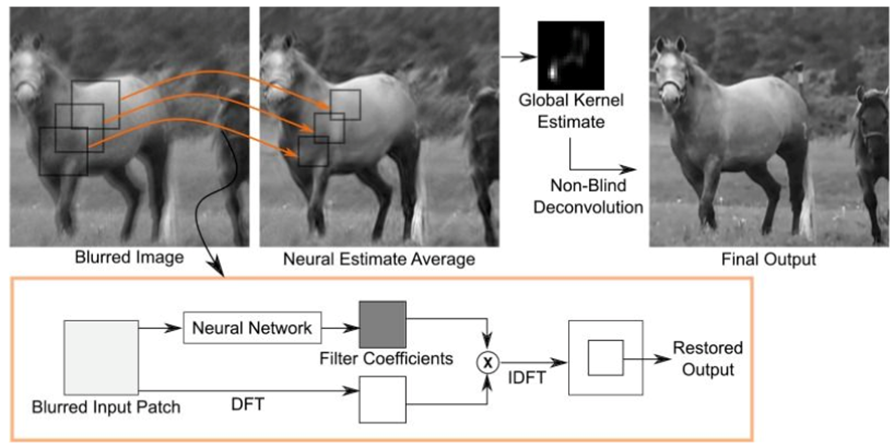
\includegraphics[width = 0.46\textwidth]{pic/non_iterative_neural_approach_pipeline.png}}
\hspace{\fill}
\subfloat[network structure]{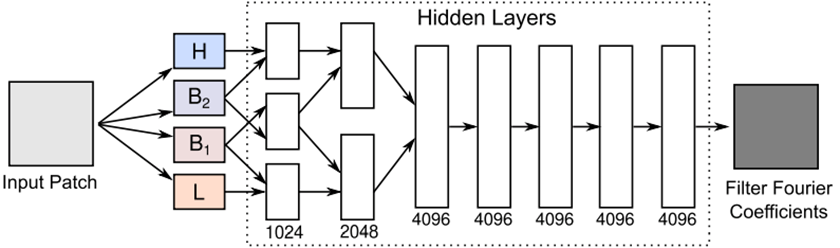
\includegraphics[width = 0.46\textwidth]{pic/non_iterative_neural_approach_structure.png}}
\hspace{\fill}
\caption{Non-iterative Neural Approach Pipeline and Network Structure}
\label{fig:non_iterative_nn}
\end{figure}
This method is non-iterative and highly parallable, which is friendly to GPU hardware.

\section{Preliminary Ideas}
After reading these papers, I find two 


% http://www.michaelshell.org/tex/ieeetran/bibtex/
\newpage
\bibliographystyle{IEEEtran}
% argument is your BibTeX string definitions and bibliography database(s)
\bibliography{reference}


% that's all folks
\end{document}


